% Options for packages loaded elsewhere
\PassOptionsToPackage{unicode}{hyperref}
\PassOptionsToPackage{hyphens}{url}
%
\documentclass[
]{article}
\usepackage{amsmath,amssymb}
\usepackage{iftex}
\ifPDFTeX
  \usepackage[T1]{fontenc}
  \usepackage[utf8]{inputenc}
  \usepackage{textcomp} % provide euro and other symbols
\else % if luatex or xetex
  \usepackage{unicode-math} % this also loads fontspec
  \defaultfontfeatures{Scale=MatchLowercase}
  \defaultfontfeatures[\rmfamily]{Ligatures=TeX,Scale=1}
\fi
\usepackage{lmodern}
\ifPDFTeX\else
  % xetex/luatex font selection
\fi
% Use upquote if available, for straight quotes in verbatim environments
\IfFileExists{upquote.sty}{\usepackage{upquote}}{}
\IfFileExists{microtype.sty}{% use microtype if available
  \usepackage[]{microtype}
  \UseMicrotypeSet[protrusion]{basicmath} % disable protrusion for tt fonts
}{}
\makeatletter
\@ifundefined{KOMAClassName}{% if non-KOMA class
  \IfFileExists{parskip.sty}{%
    \usepackage{parskip}
  }{% else
    \setlength{\parindent}{0pt}
    \setlength{\parskip}{6pt plus 2pt minus 1pt}}
}{% if KOMA class
  \KOMAoptions{parskip=half}}
\makeatother
\usepackage{xcolor}
\usepackage{color}
\usepackage{fancyvrb}
\newcommand{\VerbBar}{|}
\newcommand{\VERB}{\Verb[commandchars=\\\{\}]}
\DefineVerbatimEnvironment{Highlighting}{Verbatim}{commandchars=\\\{\}}
% Add ',fontsize=\small' for more characters per line
\newenvironment{Shaded}{}{}
\newcommand{\AlertTok}[1]{\textcolor[rgb]{1.00,0.00,0.00}{\textbf{#1}}}
\newcommand{\AnnotationTok}[1]{\textcolor[rgb]{0.38,0.63,0.69}{\textbf{\textit{#1}}}}
\newcommand{\AttributeTok}[1]{\textcolor[rgb]{0.49,0.56,0.16}{#1}}
\newcommand{\BaseNTok}[1]{\textcolor[rgb]{0.25,0.63,0.44}{#1}}
\newcommand{\BuiltInTok}[1]{\textcolor[rgb]{0.00,0.50,0.00}{#1}}
\newcommand{\CharTok}[1]{\textcolor[rgb]{0.25,0.44,0.63}{#1}}
\newcommand{\CommentTok}[1]{\textcolor[rgb]{0.38,0.63,0.69}{\textit{#1}}}
\newcommand{\CommentVarTok}[1]{\textcolor[rgb]{0.38,0.63,0.69}{\textbf{\textit{#1}}}}
\newcommand{\ConstantTok}[1]{\textcolor[rgb]{0.53,0.00,0.00}{#1}}
\newcommand{\ControlFlowTok}[1]{\textcolor[rgb]{0.00,0.44,0.13}{\textbf{#1}}}
\newcommand{\DataTypeTok}[1]{\textcolor[rgb]{0.56,0.13,0.00}{#1}}
\newcommand{\DecValTok}[1]{\textcolor[rgb]{0.25,0.63,0.44}{#1}}
\newcommand{\DocumentationTok}[1]{\textcolor[rgb]{0.73,0.13,0.13}{\textit{#1}}}
\newcommand{\ErrorTok}[1]{\textcolor[rgb]{1.00,0.00,0.00}{\textbf{#1}}}
\newcommand{\ExtensionTok}[1]{#1}
\newcommand{\FloatTok}[1]{\textcolor[rgb]{0.25,0.63,0.44}{#1}}
\newcommand{\FunctionTok}[1]{\textcolor[rgb]{0.02,0.16,0.49}{#1}}
\newcommand{\ImportTok}[1]{\textcolor[rgb]{0.00,0.50,0.00}{\textbf{#1}}}
\newcommand{\InformationTok}[1]{\textcolor[rgb]{0.38,0.63,0.69}{\textbf{\textit{#1}}}}
\newcommand{\KeywordTok}[1]{\textcolor[rgb]{0.00,0.44,0.13}{\textbf{#1}}}
\newcommand{\NormalTok}[1]{#1}
\newcommand{\OperatorTok}[1]{\textcolor[rgb]{0.40,0.40,0.40}{#1}}
\newcommand{\OtherTok}[1]{\textcolor[rgb]{0.00,0.44,0.13}{#1}}
\newcommand{\PreprocessorTok}[1]{\textcolor[rgb]{0.74,0.48,0.00}{#1}}
\newcommand{\RegionMarkerTok}[1]{#1}
\newcommand{\SpecialCharTok}[1]{\textcolor[rgb]{0.25,0.44,0.63}{#1}}
\newcommand{\SpecialStringTok}[1]{\textcolor[rgb]{0.73,0.40,0.53}{#1}}
\newcommand{\StringTok}[1]{\textcolor[rgb]{0.25,0.44,0.63}{#1}}
\newcommand{\VariableTok}[1]{\textcolor[rgb]{0.10,0.09,0.49}{#1}}
\newcommand{\VerbatimStringTok}[1]{\textcolor[rgb]{0.25,0.44,0.63}{#1}}
\newcommand{\WarningTok}[1]{\textcolor[rgb]{0.38,0.63,0.69}{\textbf{\textit{#1}}}}
\usepackage{longtable,booktabs,array}
\usepackage{calc} % for calculating minipage widths
% Correct order of tables after \paragraph or \subparagraph
\usepackage{etoolbox}
\makeatletter
\patchcmd\longtable{\par}{\if@noskipsec\mbox{}\fi\par}{}{}
\makeatother
% Allow footnotes in longtable head/foot
\IfFileExists{footnotehyper.sty}{\usepackage{footnotehyper}}{\usepackage{footnote}}
\makesavenoteenv{longtable}
\usepackage{graphicx}
\makeatletter
\def\maxwidth{\ifdim\Gin@nat@width>\linewidth\linewidth\else\Gin@nat@width\fi}
\def\maxheight{\ifdim\Gin@nat@height>\textheight\textheight\else\Gin@nat@height\fi}
\makeatother
% Scale images if necessary, so that they will not overflow the page
% margins by default, and it is still possible to overwrite the defaults
% using explicit options in \includegraphics[width, height, ...]{}
\setkeys{Gin}{width=\maxwidth,height=\maxheight,keepaspectratio}
% Set default figure placement to htbp
\makeatletter
\def\fps@figure{htbp}
\makeatother
\setlength{\emergencystretch}{3em} % prevent overfull lines
\providecommand{\tightlist}{%
  \setlength{\itemsep}{0pt}\setlength{\parskip}{0pt}}
\setcounter{secnumdepth}{-\maxdimen} % remove section numbering
\ifLuaTeX
  \usepackage{selnolig}  % disable illegal ligatures
\fi
\usepackage{bookmark}
\IfFileExists{xurl.sty}{\usepackage{xurl}}{} % add URL line breaks if available
\urlstyle{same}
\hypersetup{
  hidelinks,
  pdfcreator={LaTeX via pandoc}}

\author{}
\date{}

\begin{document}

{
\setcounter{tocdepth}{3}
\tableofcontents
}
\section{The Failure Granularity Tax: How Detailed Should Agent Failures
Be for Self-Evolving
Training?}\label{the-failure-granularity-tax-how-detailed-should-agent-failures-be-for-self-evolving-training}

\textbf{Anonymous Authors}

\subsection{Abstract}\label{abstract}

Self-evolving agents increasingly use observed failures to decide what
experience to generate next. A natural assumption is that more precise
failure diagnosis should yield better training curricula. We test this
assumption in a controlled setting and find that it is incomplete. We
introduce \textbf{failure granularity} as an independent curriculum
variable and build \textbf{GranularityBench-H8}, a CPU-executable
procedural benchmark with a strict four-level hierarchy: Global →
Capability → Failure Family → Individual Failure over eight agent
failure mechanisms. This hierarchy allows diagnostic specificity,
cross-skill transfer, task entanglement, diagnostic noise, horizon,
stochastic transition noise, training budget, and deployment
concentration to be manipulated independently.

Across \textbf{5,840 seeded training configurations}, a 100-seed causal
intervention reveals a sharp local--global trade-off. Conditioning
directly on an individual failure raises targeted state-tracking repair
by \textbf{0.197} relative to global training (95\% bootstrap CI
{[}0.182, 0.212{]}) and raises target-only success by \textbf{9.66
percentage points}, but normalized experience-support entropy falls by
\textbf{0.380}, broad held-out success falls by \textbf{23.32 points},
and external-shift success falls by \textbf{23.53 points}. The result
survives alternative support definitions including effective support,
coverage, and Jensen--Shannon divergence. An empirical phase diagram
over transfer, target prevalence, diagnostic noise, and budget shows
systematic regime changes: at diagnostic noise 0.2, fine failure
conditioning wins 16/20 transfer--prevalence cells at budget 40,
capability-level conditioning wins 16/20 at budget 80, and global
training wins 16/20 at budget 160. Under heterogeneous evaluation
distributions, however, fixed failure-conditioning strategies do not
outperform a strong difficulty curriculum.

We formalize this phenomenon as the \textbf{Failure Granularity Tax}:
finer diagnoses increase repair alignment while shrinking the support of
future experience. A discrete single-crossing result characterizes when
an intermediate abstraction is optimal. Our results argue that failure
diagnosis and curriculum specialization should be treated as distinct
design choices: knowing \emph{why} an agent failed does not imply that
future experience should collapse to that failure.

\begin{center}\rule{0.5\linewidth}{0.5pt}\end{center}

\subsection{1. Introduction}\label{introduction}

Modern agents learn in environments that are increasingly generated,
simulated, or adapted online. Synthetic task generation can supply
executable experiences at scale; adaptive schedulers can emphasize
policy-boundary or high-learning-value examples; and self-evolving
arenas can use observed capability gaps to synthesize the next round of
training tasks. These developments shift a central design problem from
\emph{whether} to adapt experience toward \emph{how} to condition that
adaptation.

Consider an agent that retrieves the correct customer identifier and
later uses a stale identifier. The same trajectory can be summarized at
several abstraction levels:

\begin{enumerate}
\def\labelenumi{\arabic{enumi}.}
\tightlist
\item
  \textbf{Global:} the agent failed;
\item
  \textbf{Capability:} the failure belongs to interaction execution;
\item
  \textbf{Family:} the failure is temporal/state-dependent;
\item
  \textbf{Failure:} the specific mechanism is state tracking.
\end{enumerate}

The finest diagnosis is informationally richest. It is therefore
tempting to generate the next training tasks specifically around state
tracking. But this changes two quantities simultaneously. It increases
\textbf{repair alignment}---the training distribution is better matched
to the diagnosed weakness---while reducing \textbf{experience
support}---the agent sees fewer neighboring mechanisms, task
compositions, and cross-skill contexts. The second effect can reduce
transfer even when local repair improves.

We call this tension the \textbf{Failure Granularity Tax}. The tax is
not the claim that fine conditioning is always bad. Rather, it is the
opportunity cost paid when diagnostic specificity collapses the support
of future experience. The optimal abstraction should therefore depend on
the deployment distribution, transfer structure, available budget, and
reliability of the diagnosis.

Existing work motivates but does not isolate this question. Curriculum
learning studies ordering and selection of training examples; automatic
curriculum methods select tasks based on progress or difficulty;
procedural RL methods prioritize levels or generate environments; and
recent agent work synthesizes tool environments, adapts task difficulty,
or schedules data around model capabilities. Our focus is orthogonal:
\textbf{holding the underlying agent-learning problem fixed, at what
abstraction level should a diagnosed failure control future experience?}

\subsubsection{1.1 Contributions}\label{contributions}

We make five contributions:

\begin{enumerate}
\def\labelenumi{\arabic{enumi}.}
\tightlist
\item
  \textbf{Failure granularity as a curriculum variable.} We separate the
  information contained in a diagnosis from the specificity of the
  training distribution induced by that diagnosis.
\item
  \textbf{GranularityBench-H8.} We introduce a fully procedural
  eight-failure benchmark with a strict nested hierarchy and independent
  controls for transfer, entanglement, diagnostic noise, transition
  stochasticity, horizon, budget, and deployment concentration.
\item
  \textbf{Causal evidence for a repair--support trade-off.} In a
  100-seed intervention, finer conditioning produces substantially
  stronger target repair but sharply lower experience support and broad
  transfer.
\item
  \textbf{An empirical granularity phase diagram.} A 4,320-configuration
  sweep demonstrates systematic shifts from fine to intermediate to
  global conditioning as training budget increases, with target
  prevalence, transfer, and noise modulating the boundary.
\item
  \textbf{A principled theory and negative results.} We give a
  single-crossing characterization of optimal granularity, show
  robustness to alternative support metrics and additional stressors,
  and report that fixed failure-conditioned curricula do not beat
  difficulty scheduling under broad heterogeneous evaluation.
\end{enumerate}

The goal is not to claim a new frontier language model.
GranularityBench-H8 deliberately removes language-model scale as a
confound so that the causal role of diagnostic abstraction can be
measured exhaustively and reproducibly on CPU.

\begin{center}\rule{0.5\linewidth}{0.5pt}\end{center}

\subsection{2. Related Work}\label{related-work}

\subsubsection{2.1 Curriculum learning and automatic task
selection}\label{curriculum-learning-and-automatic-task-selection}

Curriculum learning organizes examples or tasks to improve optimization
and generalization (Bengio et al., 2009). Teacher--Student Curriculum
Learning selects subtasks according to learning progress (Matiisen et
al., 2017), while reverse curriculum generation grows start-state
difficulty around achievable regions (Florensa et al., 2017).
Prioritized Level Replay selects procedurally generated levels using
estimated learning potential (Jiang et al., 2020). These approaches
establish that the training distribution should depend on the learner.
Our question is narrower: how much of a failure diagnosis should be used
to narrow that distribution?

\subsubsection{2.2 Environment design and procedural
generalization}\label{environment-design-and-procedural-generalization}

Unsupervised environment design, including PAIRED, treats the
environment distribution itself as an adaptive optimization object and
uses regret to generate solvable but challenging environments (Dennis et
al., 2020). This literature highlights the importance of the
relationship between training support and zero-shot transfer. Failure
granularity introduces a complementary axis: the abstraction level of
the diagnostic signal conditioning environment selection.

\subsubsection{2.3 Synthetic environments and self-evolving
agents}\label{synthetic-environments-and-self-evolving-agents}

Recent agent systems increasingly create their own training experience.
Agent-World combines scalable executable environment/task discovery with
continuous training around detected capability gaps. AutoPlay explores
interactive environments to synthesize feasible and verifiable tasks.
SYNTHAGENT jointly synthesizes tool-use tasks, mock environments,
simulated users, and rubric-based rewards, while SynthAgent refines
synthetic web tasks and trajectories. AgenticQwen uses multi-round
synthetic-data flywheels that increase reasoning and agentic task
complexity. These systems demonstrate the practical importance of
adaptive synthetic experience. They do not, however, isolate whether a
failure should condition future experience globally, at a broad
capability level, at a failure-family level, or at a specific mechanism
level.

\subsubsection{2.4 Adaptive data scheduling for
RL}\label{adaptive-data-scheduling-for-rl}

Adaptive Data Scheduling (ADS) replaces uniform RL sampling with
adaptive semantic-cluster scheduling and policy-boundary selection. Such
work asks \emph{which data are informative now}. Failure granularity
instead asks \emph{at which diagnostic abstraction should the candidate
data distribution be defined}. The two questions are complementary: a
policy-boundary selector could operate inside any granularity level.

\begin{center}\rule{0.5\linewidth}{0.5pt}\end{center}

\subsection{3. Problem Formulation}\label{problem-formulation}

Let the set of failure mechanisms be

{[} \mathcal F=\{f\_1,\ldots,f\_K\}. {]}

A failure hierarchy consists of nested partitions

{[} \Pi\_0 \preceq \Pi\_1 \preceq \cdots \preceq \Pi\_G, {]}

where each successive partition refines the previous one. For a
diagnosed failure (f), let (B\_g(f)) denote the block containing (f) at
granularity (g). A curriculum generator conditioned at level (g) samples

{[} x\sim q\_g(x\mid B\_g(f)). {]}

Finer granularity makes (B\_g(f)) smaller. This can increase the
probability that a sampled experience exercises the deficient mechanism,
but it can also reduce the diversity of neighboring skills and
compositions.

We decompose curriculum utility as

{[} J\_g = A\_g - \lambda C\_g, {]}

where (A\_g) is repair alignment and (C\_g) is a support-mismatch cost
relative to the downstream distribution. (\lambda) captures how strongly
broad transfer matters for the deployment objective.

\subsubsection{3.1 Repair alignment}\label{repair-alignment}

For target failure (f), define

{[} A\_g(f)=\mathbb E{[}\Delta c\_f\mid q\_g{]}, {]}

where (c\_f) is competence on the target failure mechanism.

\subsubsection{3.2 Experience support}\label{experience-support}

We measure support in four ways:

\begin{itemize}
\tightlist
\item
  normalized entropy (H(q\_g)/\log \textbar{}\mathcal X\textbar);
\item
  normalized effective support
  (\exp(H(q\_g))/\textbar{}\mathcal X\textbar);
\item
  empirical support coverage;
\item
  Jensen--Shannon divergence from the global training distribution.
\end{itemize}

The main experiments use normalized entropy; the remaining definitions
are robustness checks.

\subsubsection{3.3 Granularity regret}\label{granularity-regret}

For a regime (r), let (g\_r\^{}*) be the best fixed granularity. The
regret of a selected level (\hat g) is

{[} \mathrm{Regret}(\hat g;r)=R(g\_r\^{}*;r)-R(\hat g;r). {]}

This metric becomes useful when differences between fixed strategies are
small: it measures whether a controller correctly identifies the
regime-specific abstraction.

\begin{center}\rule{0.5\linewidth}{0.5pt}\end{center}

\subsection{4. Theory: Why an Interior Granularity Can Be
Optimal}\label{theory-why-an-interior-granularity-can-be-optimal}

\subsubsection{Proposition 1 --- Support contraction under nested
conditioning}\label{proposition-1-support-contraction-under-nested-conditioning}

Let (S\_g) be the support of the experience generator at granularity
(g), and assume

{[} S\_\{g+1\}\subseteq S\_g. {]}

Then the maximum possible entropy obeys

{[}
H(q\_\{g+1\})\le \log\textbar S\_\{g+1\}\textbar{}\le \log\textbar S\_g\textbar.
{]}

Thus, finer conditioning weakly decreases the maximum attainable
experience support. If refinement removes at least one experience with
positive probability and the generator assigns nonzero mass across the
coarser support, the inequality is strict.

This proposition is structural: it does not require a particular
learning algorithm. It establishes that diagnostic refinement can impose
a support cost even when the diagnosis itself is perfectly correct.

\subsubsection{Proposition 2 --- Single-crossing optimal
granularity}\label{proposition-2-single-crossing-optimal-granularity}

Order granularities from coarse to fine. Define adjacent increments

{[} a\_g=A\_\{g+1\}-A\_g,\qquad c\_g=C\_\{g+1\}-C\_g\textgreater0, {]}

and marginal alignment-to-cost ratios

{[} r\_g=\frac{a_g}{c_g}. {]}

Assume (r\_g) is strictly decreasing with (g). Then
(J\_g=A\_g-\lambda C\_g) is unimodal. Moreover, the unique optimum is
level (k) whenever

{[} r\_k \textless{} \lambda \textless{} r\_\{k-1\}, {]}

with boundary conventions (r\_\{-1\}=+\infty) and (r\_G=-\infty).

\textbf{Proof sketch.} Adjacent utility differences satisfy

{[} J\_\{g+1\}-J\_g=a\_g-\lambda c\_g=c\_g(r\_g-\lambda). {]}

Because (c\_g\textgreater0), the sign is determined by (r\_g-\lambda).
Strictly decreasing (r\_g) implies the sign can switch from positive to
negative at most once, yielding a unique interior maximizer when
(\lambda) falls between adjacent ratios. A full proof is in Appendix A.

\subsubsection{Corollary --- Deployment
concentration}\label{corollary-deployment-concentration}

If increasing target-failure prevalence reduces the effective weight on
broad-support mismatch, i.e.~(\lambda(\rho)) decreases with target
prevalence (\rho), Proposition 2 predicts a weak shift toward finer
optimal granularities as the deployment distribution concentrates around
the target mechanism.

\subsubsection{Budget interpretation}\label{budget-interpretation}

Fine curricula can have high early learning rates because a large
fraction of experiences exercise the target. Broad curricula accumulate
competence across more mechanisms and can catch up as budget increases.
Consequently, even with fixed deployment concentration, the effective
alignment-to-cost trade-off can change with budget. We test this
empirically rather than asserting monotonicity as a theorem.

\begin{center}\rule{0.5\linewidth}{0.5pt}\end{center}

\subsection{5. GranularityBench-H8}\label{granularitybench-h8}

GranularityBench-H8 is a procedural skill-acquisition environment
designed to isolate failure-conditioning granularity. It contains eight
latent mechanisms:

\begin{enumerate}
\def\labelenumi{\arabic{enumi}.}
\tightlist
\item
  tool selection;
\item
  argument grounding;
\item
  action ordering;
\item
  state tracking;
\item
  premature termination;
\item
  recovery;
\item
  constraint compliance;
\item
  verification.
\end{enumerate}

\subsubsection{5.1 Strict hierarchy}\label{strict-hierarchy}

The final benchmark uses a genuine nested hierarchy:

\begin{itemize}
\tightlist
\item
  \textbf{Global:} all eight mechanisms;
\item
  \textbf{Capability:} four mechanisms per capability;
\item
  \textbf{Family:} two mechanisms per failure family;
\item
  \textbf{Failure:} one mechanism.
\end{itemize}

For the state-tracking target used in the direct causal study:

{[} \{1,\ldots,8\} \supset \{\text{tool,arg,order,state}\} \supset
\{\text{order,state}\} \supset \{\text{state}\}. {]}

This nesting is important: each level has strictly different candidate
support.

\subsubsection{5.2 Task generation}\label{task-generation}

Each task contains a binary requirement vector (z\in\{0,1\}\^{}8),
difficulty (d), and horizon (h). A global task samples requirements
broadly. Capability-, family-, and failure-conditioned tasks
progressively restrict the mechanism set. Entanglement can introduce
additional requirements, while transition noise can add an unobserved
secondary requirement.

\subsubsection{5.3 Agent competence and
success}\label{agent-competence-and-success}

Agents maintain mechanism-level competence (c\in[0,1]\^{}8). For a task
requiring mechanisms (z), success probability is a logistic function of
required competence, task difficulty, horizon, and---where
applicable---shared representation:

{[}
p(\mathrm{success}\mid x)=\sigma!\left(\beta\left[\frac{c^\top z}{\|z\|_1}-d+s(z)\right]-\eta(h-4)\_+\right).
{]}

Updates are strongest near the learning frontier through a factor
proportional to (p(1-p)). This creates diminishing value for examples
that are either already solved or far beyond the current policy.

\subsubsection{5.4 Three representation/update
regimes}\label{three-representationupdate-regimes}

We evaluate:

\begin{itemize}
\tightlist
\item
  \textbf{Tabular/no-transfer:} only directly exercised skills are
  updated;
\item
  \textbf{Linear-sharing:} moderate structured cross-skill transfer;
\item
  \textbf{Nonlinear-sharing:} stronger state-dependent transfer with
  diminishing cross-skill gains.
\end{itemize}

These are controlled learning regimes, not claims about language-model
architectures.

\begin{center}\rule{0.5\linewidth}{0.5pt}\end{center}

\subsection{6. Curricula}\label{curricula}

We compare six curricula under identical training budgets.

\textbf{Uniform.} Broad random task sampling.

\textbf{Difficulty.} From a small candidate set, select the task whose
predicted success is closest to 0.5.

\textbf{Capability.} Diagnose failure mass and sample from the
corresponding four-mechanism capability.

\textbf{Family.} Diagnose failure mass and sample from the corresponding
two-mechanism family.

\textbf{Failure.} Sample individual failure-conditioned tasks according
to the diagnosed failure distribution.

\textbf{Random Granularity.} Randomly choose among global, capability,
family, and failure conditioning.

Diagnostic noise routes an observed failure to an incorrect mechanism
with controlled probability.

\begin{center}\rule{0.5\linewidth}{0.5pt}\end{center}

\subsection{7. Experimental Protocol}\label{experimental-protocol}

\subsubsection{7.1 Main heterogeneous-distribution
experiment}\label{main-heterogeneous-distribution-experiment}

We use 20 untouched seeds per representation regime, three regimes, six
curricula, three training rounds, and four evaluation checkpoints. This
produces 360 complete training runs and 1,440 checkpoint evaluations.

\subsubsection{7.2 Direct causal granularity
intervention}\label{direct-causal-granularity-intervention}

The central experiment uses 100 untouched seeds. The target is state
tracking. Each agent receives exactly 100 training experiences at one
fixed granularity. We then evaluate:

\begin{itemize}
\tightlist
\item
  state-repair gain;
\item
  target-only success;
\item
  broad held-out success;
\item
  external-shift success;
\item
  support entropy;
\item
  support coverage;
\item
  mean all-skill gain.
\end{itemize}

\subsubsection{7.3 Empirical phase
diagram}\label{empirical-phase-diagram}

We sweep:

{[} \text{transfer}\in\{0,.25,.5,.75,1\}, {]}

{[} \text{target prevalence}\in\{.25,.5,.75,1\}, {]}

{[} \text{budget}\in\{40,80,160\}, {]}

{[} \text{diagnostic noise}\in\{0,.2,.4\}. {]}

With six independent seeds and four granularities, this contributes
4,320 seeded training configurations.

\subsubsection{7.4 Robustness and stress
tests}\label{robustness-and-stress-tests}

We additionally test:

\begin{itemize}
\tightlist
\item
  alternative support definitions on 40 seeds;
\item
  entanglement from 0 to 1;
\item
  horizon from 2 to 16;
\item
  stochastic transition noise from 0 to 0.4;
\item
  100-seed direct replication with paired bootstrap and Wilcoxon tests.
\end{itemize}

The full final suite contains \textbf{5,840 seeded training
configurations} excluding plotting and analysis-only computations.

\subsubsection{7.5 Statistics}\label{statistics}

Primary causal comparisons use paired differences over seeds,
10,000-sample bootstrap confidence intervals, paired t-tests, and
Wilcoxon signed-rank tests as a nonparametric robustness check. Main
multi-method comparisons receive Holm correction. We report effect sizes
and confidence intervals rather than relying on significance alone.

\begin{center}\rule{0.5\linewidth}{0.5pt}\end{center}

\subsection{8. Results}\label{results}

\subsubsection{8.1 Under a broad heterogeneous distribution, fixed
granularity is not a strong
winner}\label{under-a-broad-heterogeneous-distribution-fixed-granularity-is-not-a-strong-winner}

\begin{longtable}[]{@{}lrr@{}}
\toprule\noalign{}
Method & Held-out & External shift \\
\midrule\noalign{}
\endhead
\bottomrule\noalign{}
\endlastfoot
Difficulty & \textbf{87.89\%} & \textbf{84.01\%} \\
Random granularity & 87.83\% & 83.96\% \\
Capability & 87.81\% & 83.96\% \\
Uniform & 87.81\% & 83.92\% \\
Family & 87.76\% & 83.87\% \\
Failure & 87.74\% & 83.86\% \\
\end{longtable}

The differences are small. After Holm correction, no pairwise comparison
establishes a robust advantage of failure-conditioned training over the
difficulty baseline. This null result matters: failure information alone
does not imply broad-distribution gains.

\subsubsection{8.2 Fine conditioning strongly improves local repair but
collapses broad
support}\label{fine-conditioning-strongly-improves-local-repair-but-collapses-broad-support}

\begin{figure}
\centering
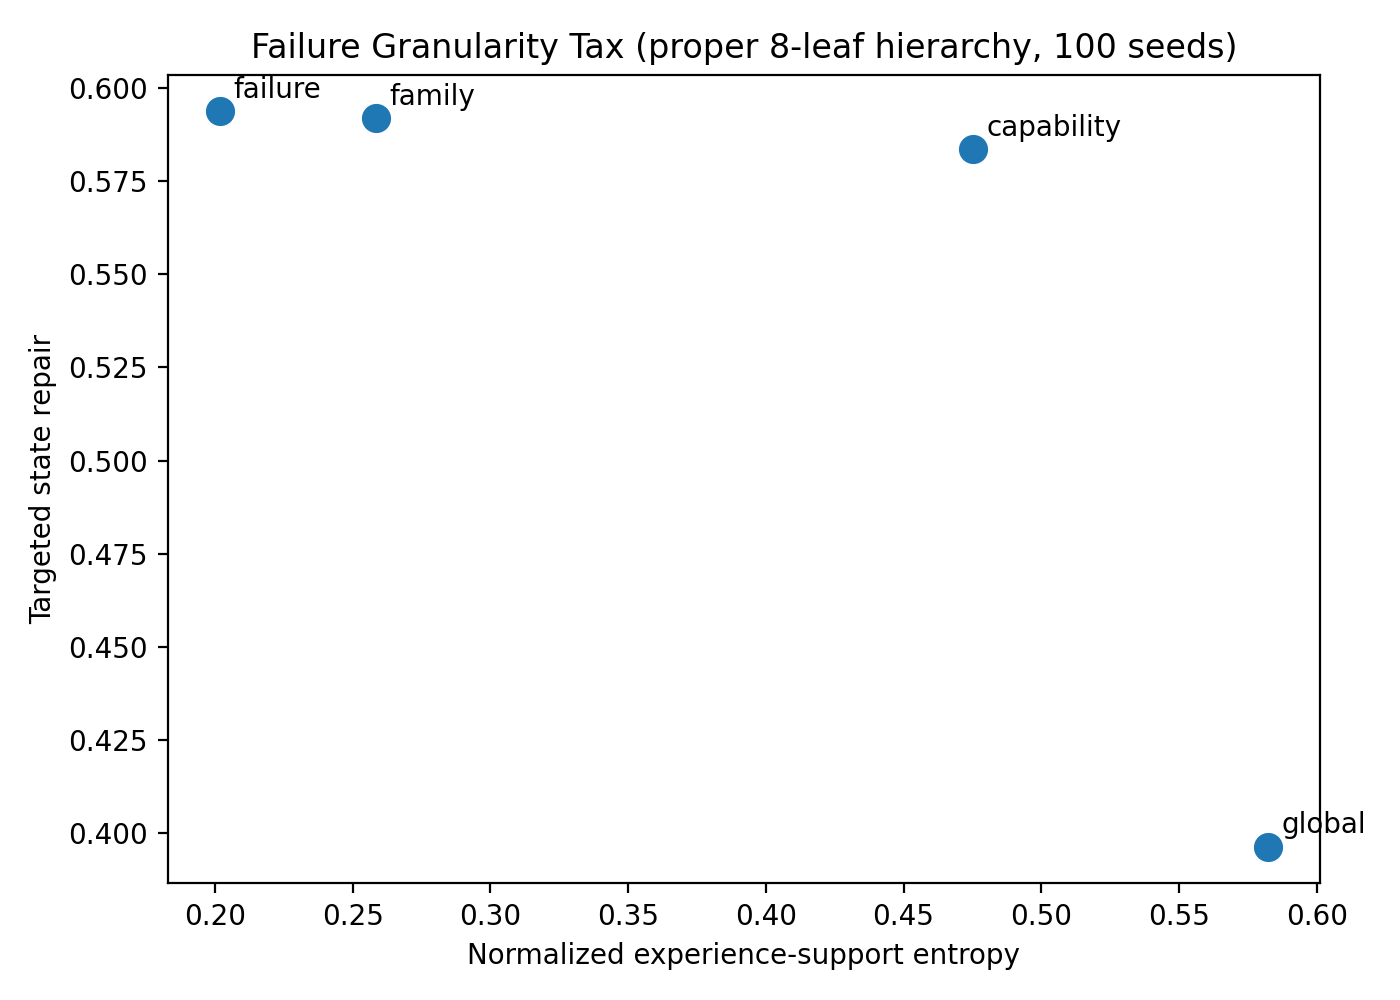
\includegraphics{figures/fig_h8_tax.png}
\caption{Direct repair-support trade-off across the four nested
granularity levels.}
\end{figure}

The 100-seed intervention gives the central result.

\begin{longtable}[]{@{}
  >{\raggedright\arraybackslash}p{(\columnwidth - 12\tabcolsep) * \real{0.1111}}
  >{\raggedleft\arraybackslash}p{(\columnwidth - 12\tabcolsep) * \real{0.1481}}
  >{\raggedleft\arraybackslash}p{(\columnwidth - 12\tabcolsep) * \real{0.1481}}
  >{\raggedleft\arraybackslash}p{(\columnwidth - 12\tabcolsep) * \real{0.1481}}
  >{\raggedleft\arraybackslash}p{(\columnwidth - 12\tabcolsep) * \real{0.1481}}
  >{\raggedleft\arraybackslash}p{(\columnwidth - 12\tabcolsep) * \real{0.1481}}
  >{\raggedleft\arraybackslash}p{(\columnwidth - 12\tabcolsep) * \real{0.1481}}@{}}
\toprule\noalign{}
\begin{minipage}[b]{\linewidth}\raggedright
Granularity
\end{minipage} & \begin{minipage}[b]{\linewidth}\raggedleft
Support entropy
\end{minipage} & \begin{minipage}[b]{\linewidth}\raggedleft
Coverage
\end{minipage} & \begin{minipage}[b]{\linewidth}\raggedleft
State repair
\end{minipage} & \begin{minipage}[b]{\linewidth}\raggedleft
Target-only success
\end{minipage} & \begin{minipage}[b]{\linewidth}\raggedleft
Broad held-out
\end{minipage} & \begin{minipage}[b]{\linewidth}\raggedleft
External
\end{minipage} \\
\midrule\noalign{}
\endhead
\bottomrule\noalign{}
\endlastfoot
Global & \textbf{0.582} & \textbf{0.133} & 0.396 & 72.30\% &
\textbf{72.47\%} & \textbf{67.46\%} \\
Capability & 0.475 & 0.075 & 0.583 & \textbf{83.47\%} & 63.51\% &
58.93\% \\
Family & 0.258 & 0.038 & 0.592 & 81.97\% & 50.38\% & 45.61\% \\
Failure & \textbf{0.202} & \textbf{0.035} & \textbf{0.594} & 81.97\% &
49.15\% & 43.93\% \\
\end{longtable}

Relative to Global, individual Failure conditioning changes:

{[} \Delta \mathrm{StateRepair}=+0.197 {]}

with 95\% bootstrap CI {[}0.182, 0.212{]}, while

{[} \Delta \mathrm{SupportEntropy}=-0.380 {]}

(CI {[}-0.386, -0.374{]}),

{[} \Delta \mathrm{Heldout}=-23.32~\mathrm{pp} {]}

(CI {[}-23.97, -22.67{]}), and

{[} \Delta \mathrm{External}=-23.53~\mathrm{pp} {]}

(CI {[}-24.19, -22.86{]}). All paired tests are highly significant.

Importantly, the finest curriculum is \textbf{not} best even on
target-only success: Capability reaches 83.47\%, about 1.5 points above
Family and Failure. This is a concrete intermediate-granularity effect.
Fine conditioning attains the highest direct state-repair coefficient,
but neighboring skills remain useful even when deployment is entirely
state-focused.

\subsubsection{8.3 The tax is not an artifact of
entropy}\label{the-tax-is-not-an-artifact-of-entropy}

We repeat the support analysis with effective support, raw coverage, and
Jensen--Shannon divergence from Global. Mean effective support falls
from 0.100 under Global to 0.054 under Capability, 0.016 under Family,
and 0.012 under Failure. Across seed-level observations, effective
support correlates strongly with broad evaluation performance (Spearman
(\rho=0.833), (p\textless10\^{}\{-41\})); Jensen--Shannon divergence
correlates negatively ((\rho=-0.807), (p\textless10\^{}\{-37\})).
Meanwhile, support entropy correlates negatively with state repair
((\rho=-0.584)), exactly reflecting the local-repair/broad-support
trade-off.

\subsubsection{8.4 A granularity phase transition appears as budget
changes}\label{a-granularity-phase-transition-appears-as-budget-changes}

\begin{figure}
\centering
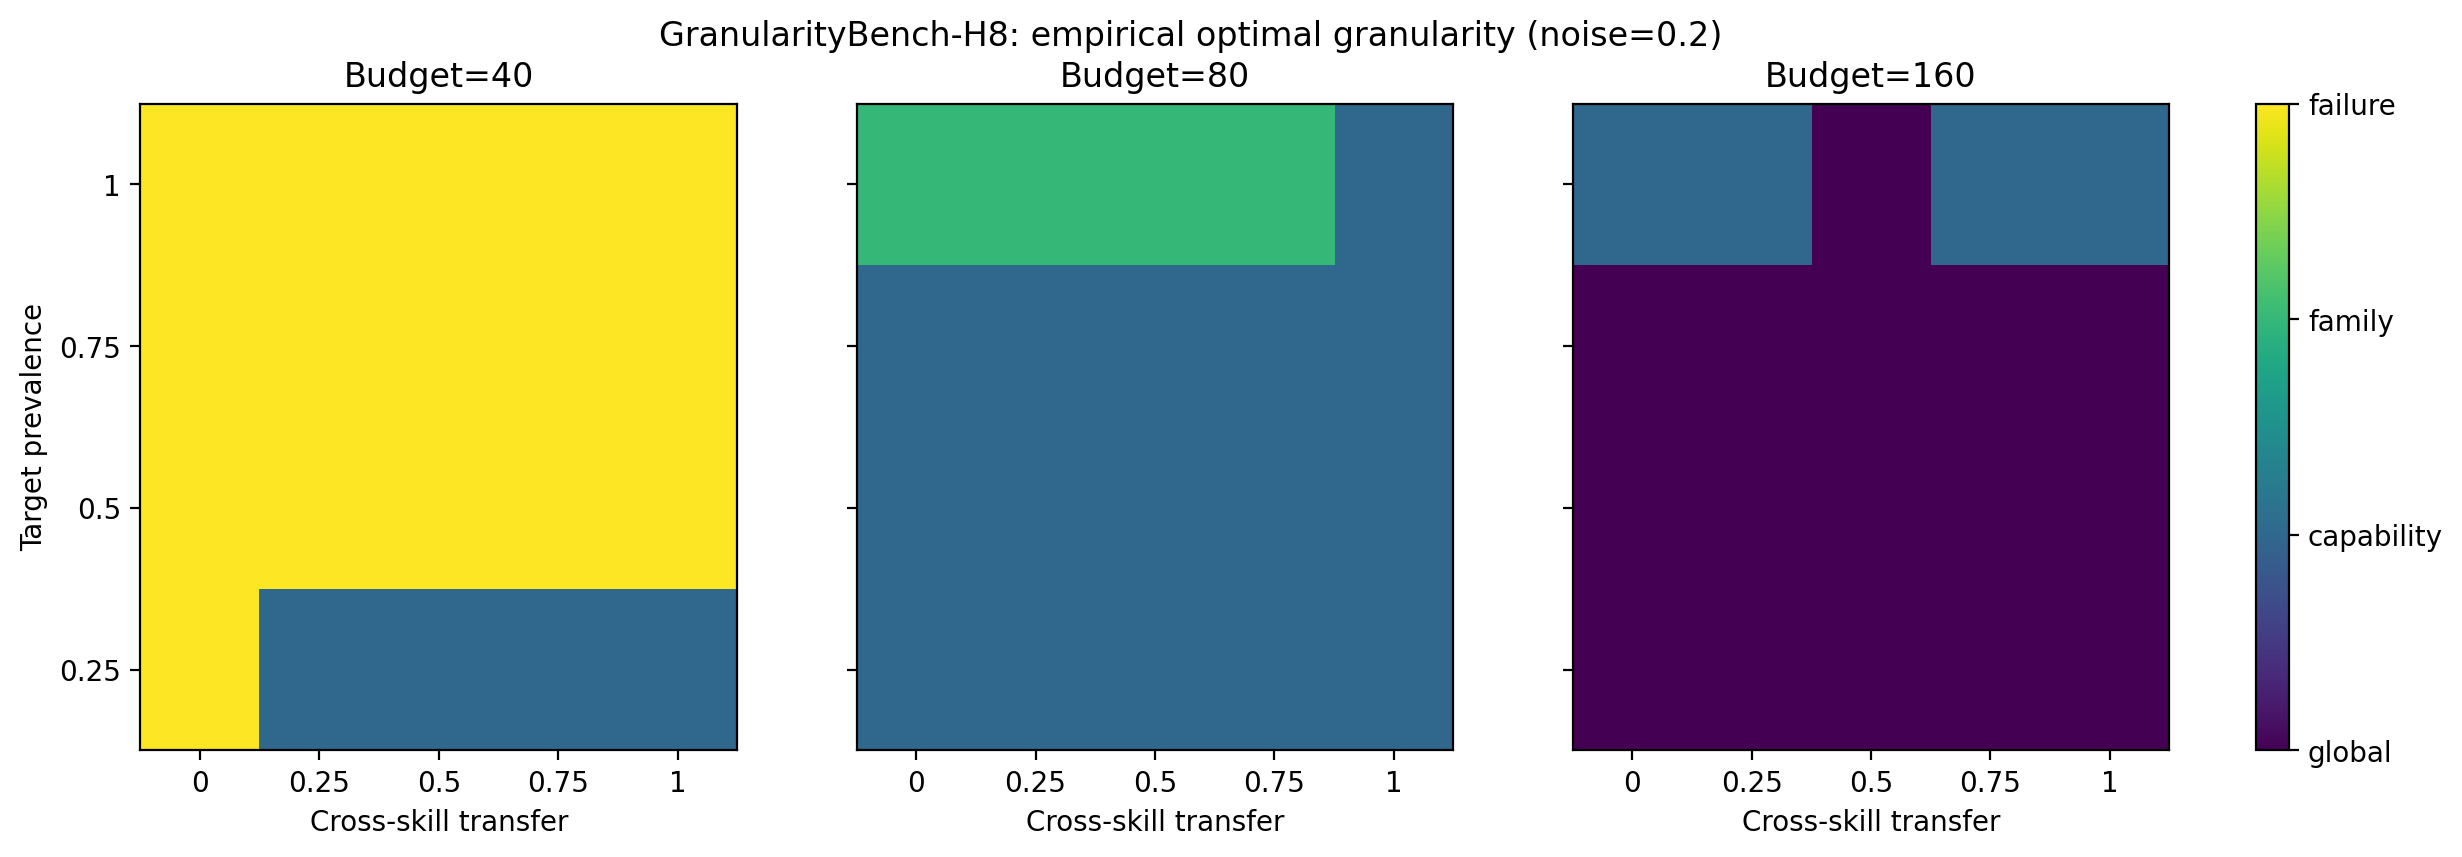
\includegraphics{figures/fig_h8_phase.png}
\caption{Empirical optimal granularity over cross-skill transfer and
target prevalence at three budgets, with diagnostic noise fixed at 0.2.}
\end{figure}

The empirical phase diagram is the strongest regime-level result. At
diagnostic noise 0.2:

\begin{itemize}
\tightlist
\item
  \textbf{Budget 40:} Failure wins 16/20 transfer × prevalence cells;
  Capability wins 4/20.
\item
  \textbf{Budget 80:} Capability wins 16/20; Family wins 4/20.
\item
  \textbf{Budget 160:} Global wins 16/20; Capability wins 4/20.
\end{itemize}

The qualitative transition is also visible at diagnostic noise 0 and
0.4. At zero noise, Failure wins 80\% of low-budget cells, Capability
wins 65\% of medium-budget cells, and Global wins 100\% of high-budget
cells. At noise 0.4, Failure wins 80\% at low budget, Capability 70\% at
medium budget, and Global 80\% at high budget.

Thus, no single abstraction is universally optimal. Fine conditioning is
most valuable when training opportunities are scarce; broader
conditioning dominates once sufficient budget allows the agent to
benefit from neighboring skills and support coverage.

\subsubsection{8.5 Target prevalence moves the
boundary}\label{target-prevalence-moves-the-boundary}

Within a fixed budget, increased target prevalence generally makes
narrower curricula more competitive. For example, at noise 0.2 and
budget 80, Capability wins most cells at 25--75\% target prevalence,
while Family wins four of the five transfer settings at 100\%
prevalence. At budget 160, Global dominates low-to-moderate target
prevalence while Capability becomes competitive at fully concentrated
deployment.

This pattern is consistent with the single-crossing interpretation: as
the downstream objective concentrates on one region of the failure
hierarchy, the effective cost of reduced global support falls.

\subsubsection{8.6 Entanglement, horizon, and
stochasticity}\label{entanglement-horizon-and-stochasticity}

Stress tests refine rather than overturn the main conclusion. At 50\%
target prevalence, Capability is usually the strongest intermediate
level across horizons 2--16. Increasing entanglement eventually benefits
broader training: at maximal entanglement, Global reaches 73.17\%
compared with Capability at 71.47\%. Transition noise increases the
value of broad support, although Capability remains strongest in the
tested 50\%-prevalence slice. Longer horizons lower absolute success but
do not induce a clean granularity phase transition.

These mixed outcomes are reported as such; we do not claim that every
nuisance variable monotonically shifts the optimum.

\begin{center}\rule{0.5\linewidth}{0.5pt}\end{center}

\subsection{9. Discussion}\label{discussion}

\subsubsection{9.1 Diagnosis and training specialization are different
decisions}\label{diagnosis-and-training-specialization-are-different-decisions}

A detailed diagnosis can be useful for analysis without implying that
the next training batch should be equally detailed. The direct
experiment makes this distinction explicit. Individual failure
conditioning repairs the diagnosed skill more strongly, but broad
performance deteriorates because training support collapses.

This suggests a two-stage design for future self-evolving systems:

\begin{enumerate}
\def\labelenumi{\arabic{enumi}.}
\tightlist
\item
  infer the most accurate failure representation available;
\item
  independently choose the granularity at which that information should
  shape training.
\end{enumerate}

Conflating the two steps implicitly assumes that maximal diagnostic
precision is also maximal curriculum precision. Our results show this
assumption can fail dramatically.

\subsubsection{9.2 Why Capability is often a strong
compromise}\label{why-capability-is-often-a-strong-compromise}

Capability-level conditioning retains four related mechanisms in
GranularityBench-H8. It therefore places substantial probability on the
target while preserving enough neighboring structure to learn
transferable competence. In the direct intervention it achieves the
highest target-only success, even though Failure produces slightly
higher raw target-mechanism repair. This distinction is important:
deployment success depends on compositions of mechanisms, not merely the
scalar competence of one leaf.

\subsubsection{9.3 Why the optimum changes with
budget}\label{why-the-optimum-changes-with-budget}

At low budget, broad sampling wastes scarce interactions on non-target
mechanisms. Fine failure conditioning therefore wins most phase cells.
At high budget, broad curricula eventually acquire both the target and
complementary mechanisms while avoiding support collapse. The phase map
makes this transition visible without requiring a new adaptive
controller.

\subsubsection{9.4 Implications for synthetic RL
systems}\label{implications-for-synthetic-rl-systems}

Recent synthetic-agent pipelines often possess richer diagnostic signals
than they use. The implication of this paper is not ``ignore
diagnosis,'' but ``do not equate diagnosis detail with data-distribution
detail.'' A practical system could estimate the transfer value of
neighboring failures, maintain a support floor, or adapt abstraction as
budget changes. Those extensions should be validated on real LLM agents
before being treated as production prescriptions.

\begin{center}\rule{0.5\linewidth}{0.5pt}\end{center}

\subsection{10. Limitations}\label{limitations}

The paper is intentionally controlled, and its claims are
correspondingly bounded.

\textbf{No language model.} GranularityBench-H8 is not Qwen, Llama,
Claude, GPT, or a natural-language tool-use benchmark. It abstracts away
token generation, tool-schema parsing, prompt sensitivity, optimizer
instability, and emergent representation learning.

\textbf{Designed hierarchy.} The eight-failure hierarchy is semantically
motivated and the transfer structure favors stronger sharing within
families/capabilities. The phase sweep varies transfer strength but does
not exhaust arbitrary transfer graphs.

\textbf{Simplified learning dynamics.} Competence updates are
interpretable proxies, not full policy-gradient optimization. Three
update regimes provide robustness to sharing assumptions, but not
architectural realism.

\textbf{Procedural evaluation.} The external shift changes diversity,
horizon, and transition noise within the same simulator family. It is
not an independent real-world benchmark.

\textbf{No universal monotonicity claim.} Diagnostic noise, horizon, and
transition stochasticity do not each create a clean one-dimensional
transition. The supported claim is the repair--support trade-off and
regime dependence, not a universal rule for every axis.

These limitations make external LLM validation the clearest next step,
but they do not invalidate the causal result within the controlled
system.

\begin{center}\rule{0.5\linewidth}{0.5pt}\end{center}

\subsection{11. Broader Impact}\label{broader-impact}

Adaptive synthetic training can reduce annotation cost and improve agent
reliability, but overly narrow failure-driven curricula may create blind
spots: the system may become excellent at a recently observed failure
while losing breadth on less frequently sampled behaviors. The Failure
Granularity Tax therefore has a safety-relevant interpretation: targeted
repair should be accompanied by coverage monitoring. GranularityBench-H8
itself contains no personal data and uses no external services or
proprietary models.

\begin{center}\rule{0.5\linewidth}{0.5pt}\end{center}

\subsection{12. Conclusion}\label{conclusion}

More precise failure diagnosis is not automatically better training
supervision. In a strict eight-failure hierarchy, fine conditioning
strongly improves local repair while shrinking experience support enough
to damage broad and shifted performance. The best granularity changes
systematically with training budget and deployment concentration:
low-budget regimes favor fine targeting, intermediate regimes favor
capability-level abstraction, and high-budget regimes favor broad
training. We formalize this tension as the \textbf{Failure Granularity
Tax}.

The central design principle is simple:

\begin{quote}
\textbf{Diagnose failures as precisely as possible, but specialize
training only as finely as the downstream transfer objective can
afford.}
\end{quote}

\begin{center}\rule{0.5\linewidth}{0.5pt}\end{center}

\section{Appendix}\label{appendix}

\subsection{Appendix A. Proofs}\label{appendix-a.-proofs}

\subsubsection{A.1 Proof of Proposition
1}\label{a.1-proof-of-proposition-1}

For any distribution (q) supported on a finite set (S), Shannon entropy
satisfies (H(q)\le \log \textbar S\textbar), with equality iff (q) is
uniform over (S). Under nested conditioning, (S\_\{g+1\}\subseteq S\_g),
hence (\textbar S\_\{g+1\}\textbar{}\le \textbar S\_g\textbar) and
therefore

{[}
H(q\_\{g+1\})\le \log\textbar S\_\{g+1\}\textbar{}\le \log\textbar S\_g\textbar.
{]}

If refinement removes at least one support element and the coarser
generator can assign positive mass to it, the maximum attainable entropy
strictly decreases.

\subsubsection{A.2 Proof of Proposition
2}\label{a.2-proof-of-proposition-2}

Let

{[} J\_g=A\_g-\lambda C\_g. {]}

Then

{[}
J\_\{g+1\}-J\_g=(A\_\{g+1\}-A\_g)-\lambda(C\_\{g+1\}-C\_g)=a\_g-\lambda c\_g.
{]}

Because (c\_g\textgreater0),

{[}
\operatorname{sign}(J\_\{g+1\}-J\_g)=\operatorname{sign}(r\_g-\lambda),
{]}

where (r\_g=a\_g/c\_g). If (r\_g) is strictly decreasing, the sequence
(r\_g-\lambda) can cross zero at most once. Therefore the utility
sequence first increases and then decreases, or is monotone at a
boundary. If

{[} r\_k\textless{}\lambda\textless r\_\{k-1\}, {]}

then increments are positive up through (k-1) and negative from (k)
onward, so (k) is the unique maximizer. □

\subsubsection{A.3 Corollary on target
prevalence}\label{a.3-corollary-on-target-prevalence}

Suppose the downstream objective is

{[} R\_\rho=\rho R\_\{target\}+(1-\rho)R\_\{broad\}, {]}

and increasing (\rho) decreases the effective support penalty
(\lambda(\rho)). The threshold rule in Proposition 2 then implies that
crossing to smaller (\lambda) values weakly shifts the optimum toward
levels with larger (g), i.e.~finer conditioning.

\subsubsection{A.4 What the theorem does and does not
assert}\label{a.4-what-the-theorem-does-and-does-not-assert}

The theorem does \textbf{not} assert that empirical alignment must rise
monotonically at every adjacent level. In fact, target-only success
peaks at Capability in our main intervention. The theorem provides
sufficient conditions for an interior optimum and a language for
interpreting the observed phase transitions. The empirical result is
stronger than a schematic monotonic story precisely because
neighboring-skill transfer can make an intermediate abstraction
outperform the finest one even on target-concentrated evaluation.

\begin{center}\rule{0.5\linewidth}{0.5pt}\end{center}

\subsection{Appendix B. Failure
Hierarchy}\label{appendix-b.-failure-hierarchy}

\begin{longtable}[]{@{}llr@{}}
\toprule\noalign{}
Level & Target-state block & Cardinality \\
\midrule\noalign{}
\endhead
\bottomrule\noalign{}
\endlastfoot
Global & all eight failures & 8 \\
Capability & tool, argument, ordering, state & 4 \\
Family & ordering, state & 2 \\
Failure & state & 1 \\
\end{longtable}

The second capability contains termination, recovery, constraint, and
verification. Families are \{tool, argument\}, \{ordering, state\},
\{termination, recovery\}, and \{constraint, verification\}.

\begin{center}\rule{0.5\linewidth}{0.5pt}\end{center}

\subsection{Appendix C. Procedural
Generator}\label{appendix-c.-procedural-generator}

Each generated task contains:

\begin{itemize}
\tightlist
\item
  a non-empty requirement mask over eight mechanisms;
\item
  difficulty sampled from a bounded beta-derived distribution;
\item
  Poisson-distributed horizon;
\item
  optional entangled requirements;
\item
  optional stochastic transition requirement.
\end{itemize}

Global generation samples broadly across all failures. Capability
generation samples inside one four-leaf block, Family inside one
two-leaf block, and Failure around one leaf with optional entanglement.

\begin{center}\rule{0.5\linewidth}{0.5pt}\end{center}

\subsection{Appendix D. Learning
Regimes}\label{appendix-d.-learning-regimes}

\textbf{Tabular.} Directly required mechanisms update; no cross-skill
transfer.

\textbf{Linear-sharing.} Required mechanisms update directly and produce
moderate transfer proportional to hierarchical affinity.

\textbf{Nonlinear-sharing.} Transfer is stronger when the receiving
skill remains weak, yielding diminishing cross-skill gains.

The hierarchy affinity is highest within a family, lower within a
capability, and lowest across capabilities. Transfer strength is
multiplied by the experimental transfer coefficient.

\begin{center}\rule{0.5\linewidth}{0.5pt}\end{center}

\subsection{Appendix E. Curriculum
Pseudocode}\label{appendix-e.-curriculum-pseudocode}

\begin{Shaded}
\begin{Highlighting}[]
\NormalTok{Input: agent π, hierarchy H, method m, budget B}
\NormalTok{Diagnose failure distribution d from broad rollouts}
\NormalTok{for b = 1 ... B:}
\NormalTok{    if m = Uniform:}
\NormalTok{        x ← sample\_global()}
\NormalTok{    if m = Difficulty:}
\NormalTok{        C ← sample\_global\_candidates(5)}
\NormalTok{        x ← argmin\_x |Pπ(success|x) {-} 0.5|}
\NormalTok{    if m = Capability:}
\NormalTok{        c ← sample capability proportional to failure mass d}
\NormalTok{        x ← sample\_from\_capability(c)}
\NormalTok{    if m = Family:}
\NormalTok{        f ← sample family proportional to failure mass d}
\NormalTok{        x ← sample\_from\_family(f)}
\NormalTok{    if m = Failure:}
\NormalTok{        k ← sample individual failure proportional to d}
\NormalTok{        x ← sample\_from\_failure(k)}
\NormalTok{    if m = RandomGranularity:}
\NormalTok{        g ← Uniform\{Global, Capability, Family, Failure\}}
\NormalTok{        x ← sample\_from\_level(g)}
\NormalTok{    update π on x}
\end{Highlighting}
\end{Shaded}

\begin{center}\rule{0.5\linewidth}{0.5pt}\end{center}

\subsection{Appendix F. Experiment
Inventory}\label{appendix-f.-experiment-inventory}

\begin{longtable}[]{@{}lr@{}}
\toprule\noalign{}
Component & Training configurations \\
\midrule\noalign{}
\endhead
\bottomrule\noalign{}
\endlastfoot
Main heterogeneous study & 360 \\
Direct causal intervention & 400 \\
Empirical phase diagram & 4,320 \\
Entanglement/horizon/stochasticity stress & 600 \\
Alternative support metrics & 160 \\
\textbf{Total} & \textbf{5,840} \\
\end{longtable}

The main study additionally logs four checkpoints per run, producing
1,440 checkpoint evaluations.

\begin{center}\rule{0.5\linewidth}{0.5pt}\end{center}

\subsection{Appendix G. Full Direct-Intervention
Statistics}\label{appendix-g.-full-direct-intervention-statistics}

Failure minus Global:

\begin{longtable}[]{@{}lrrr@{}}
\toprule\noalign{}
Metric & Difference & 95\% bootstrap CI & paired t p \\
\midrule\noalign{}
\endhead
\bottomrule\noalign{}
\endlastfoot
Support entropy & -0.380 & {[}-0.386, -0.374{]} & 1.08e-109 \\
State repair & +0.197 & {[}0.182, 0.212{]} & 5.08e-46 \\
Broad held-out & -23.32 pp & {[}-23.97, -22.67{]} & 1.62e-85 \\
External shift & -23.53 pp & {[}-24.19, -22.86{]} & 9.54e-85 \\
Target-only success & +9.66 pp & {[}8.42, 10.94{]} & 2.16e-27 \\
\end{longtable}

Failure vs Family shows no meaningful state-repair gain (difference
0.0019; CI includes zero) but does reduce broad and external success.
This is further evidence that maximal specificity can incur support cost
without additional local repair.

\begin{center}\rule{0.5\linewidth}{0.5pt}\end{center}

\subsection{Appendix H. Alternative Support
Metrics}\label{appendix-h.-alternative-support-metrics}

\begin{figure}
\centering
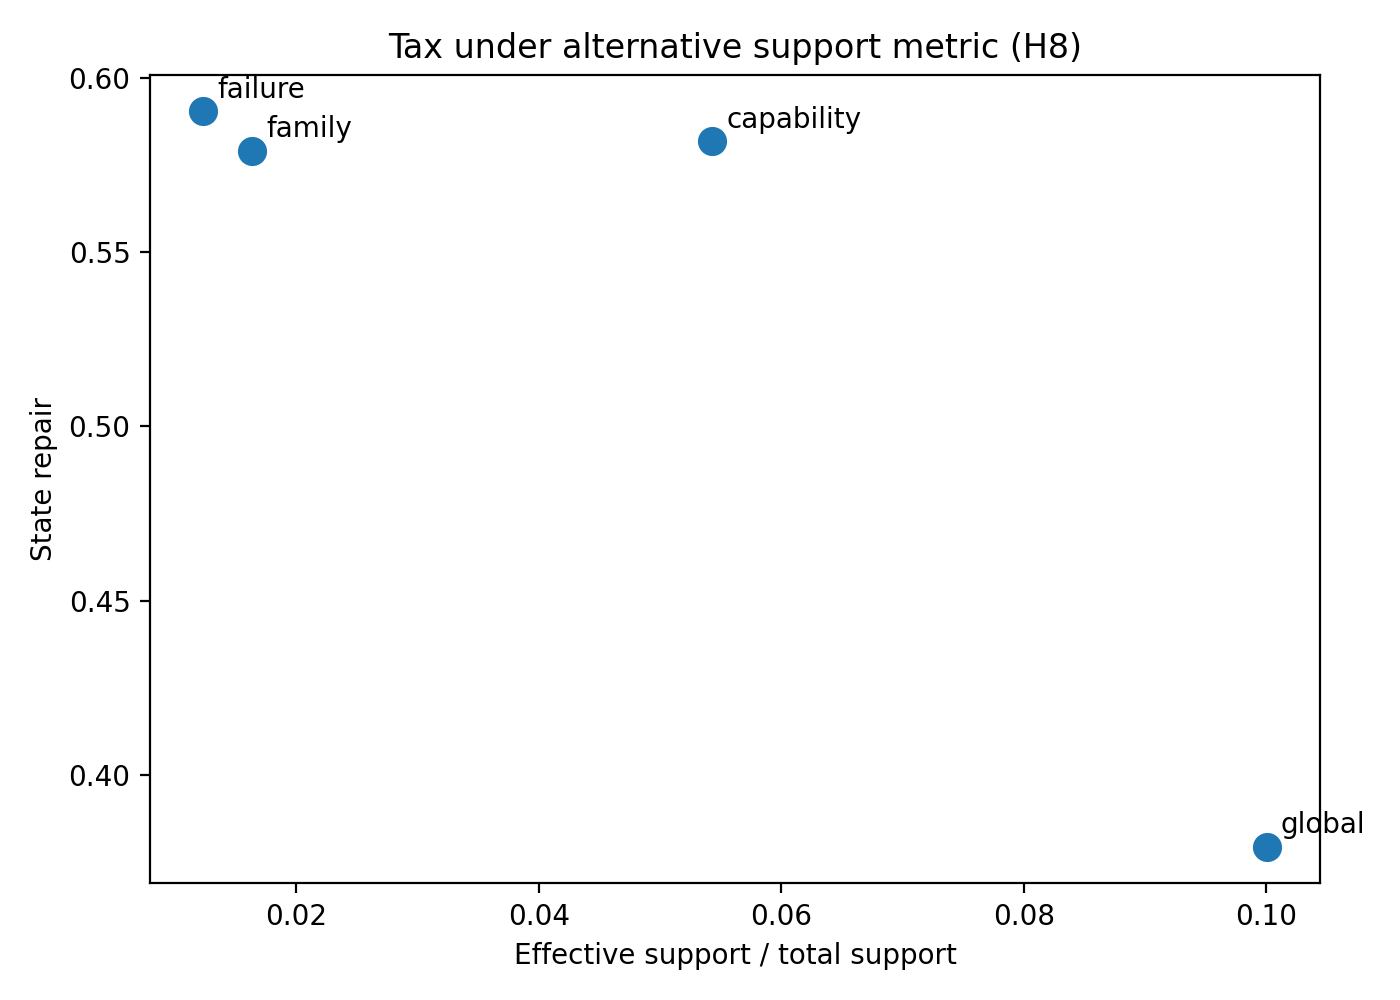
\includegraphics{figures/fig_h8_support_alt.png}
\caption{The local-repair/broad-support trade-off persists when support
is measured by normalized effective support rather than entropy.}
\end{figure}

\begin{longtable}[]{@{}
  >{\raggedright\arraybackslash}p{(\columnwidth - 10\tabcolsep) * \real{0.1304}}
  >{\raggedleft\arraybackslash}p{(\columnwidth - 10\tabcolsep) * \real{0.1739}}
  >{\raggedleft\arraybackslash}p{(\columnwidth - 10\tabcolsep) * \real{0.1739}}
  >{\raggedleft\arraybackslash}p{(\columnwidth - 10\tabcolsep) * \real{0.1739}}
  >{\raggedleft\arraybackslash}p{(\columnwidth - 10\tabcolsep) * \real{0.1739}}
  >{\raggedleft\arraybackslash}p{(\columnwidth - 10\tabcolsep) * \real{0.1739}}@{}}
\toprule\noalign{}
\begin{minipage}[b]{\linewidth}\raggedright
Level
\end{minipage} & \begin{minipage}[b]{\linewidth}\raggedleft
Entropy
\end{minipage} & \begin{minipage}[b]{\linewidth}\raggedleft
Effective support
\end{minipage} & \begin{minipage}[b]{\linewidth}\raggedleft
Coverage
\end{minipage} & \begin{minipage}[b]{\linewidth}\raggedleft
JS from Global
\end{minipage} & \begin{minipage}[b]{\linewidth}\raggedleft
Broad eval
\end{minipage} \\
\midrule\noalign{}
\endhead
\bottomrule\noalign{}
\endlastfoot
Global & 0.584 & 0.100 & 0.134 & 0.000 & 72.23\% \\
Capability & 0.474 & 0.054 & 0.073 & 0.524 & 68.19\% \\
Family & 0.257 & 0.016 & 0.038 & 0.671 & 58.03\% \\
Failure & 0.206 & 0.012 & 0.035 & 0.706 & 57.44\% \\
\end{longtable}

Seed-level Spearman correlations:

\begin{itemize}
\tightlist
\item
  effective support vs broad evaluation: (\rho=0.833);
\item
  coverage vs broad evaluation: (\rho=0.819);
\item
  JS divergence from Global vs broad evaluation: (\rho=-0.807);
\item
  normalized entropy vs state repair: (\rho=-0.584).
\end{itemize}

All have (p\textless10\^{}\{-13\}), and the broad-evaluation
correlations are below (10\^{}\{-37\}).

\begin{center}\rule{0.5\linewidth}{0.5pt}\end{center}

\subsection{Appendix I. Empirical Phase
Diagram}\label{appendix-i.-empirical-phase-diagram}

At diagnostic noise 0.2, the fraction of transfer × prevalence cells won
is:

\begin{longtable}[]{@{}rrrrr@{}}
\toprule\noalign{}
Budget & Global & Capability & Family & Failure \\
\midrule\noalign{}
\endhead
\bottomrule\noalign{}
\endlastfoot
40 & 0.00 & 0.20 & 0.00 & \textbf{0.80} \\
80 & 0.00 & \textbf{0.80} & 0.20 & 0.00 \\
160 & \textbf{0.80} & 0.20 & 0.00 & 0.00 \\
\end{longtable}

At zero noise the corresponding dominant fractions are Failure 0.80,
Capability 0.65, and Global 1.00. At noise 0.4 they are Failure 0.80,
Capability 0.70, and Global 0.80.

The phase diagram is descriptive rather than a universal law: some cells
have small winner margins, particularly near boundaries.

\begin{center}\rule{0.5\linewidth}{0.5pt}\end{center}

\subsection{Appendix J. Stress Tests}\label{appendix-j.-stress-tests}

Representative stress-test figures are included in
\texttt{figures/fig\_h8\_entangle.png},
\texttt{figures/fig\_h8\_horizon.png}, and
\texttt{figures/fig\_h8\_transition\_noise.png}.

\subsubsection{J.1 Entanglement}\label{j.1-entanglement}

At 50\% target prevalence, Capability leads for entanglement 0--0.75. At
maximal entanglement, Global becomes best (73.17\%) versus Capability
(71.47\%), illustrating that highly compositional tasks can reward
broader support.

\subsubsection{J.2 Horizon}\label{j.2-horizon}

Capability remains strongest across horizons 2, 4, 8, and 12. At horizon
16 all methods degrade; Capability remains ahead at 68.17\%. Horizon
therefore affects difficulty more reliably than optimal granularity in
this slice.

\subsubsection{J.3 Transition noise}\label{j.3-transition-noise}

Capability remains strongest from transition noise 0 to 0.4, while
Global closes much of the gap as stochasticity increases. We therefore
retain this as a robustness result rather than claiming a
stochasticity-driven phase transition.

\begin{center}\rule{0.5\linewidth}{0.5pt}\end{center}

\subsection{Appendix K. Main Multi-Method Statistical
Result}\label{appendix-k.-main-multi-method-statistical-result}

The broad-distribution differences among curricula are small. In the
Linear and Nonlinear regimes, uncorrected tests occasionally favor
Difficulty over Failure or Uniform by roughly 0.1--0.17 percentage
points, but no comparison survives the global Holm correction. The
correct interpretation is a null method result under heterogeneous
deployment, not a hidden positive claim for any failure abstraction.

\begin{center}\rule{0.5\linewidth}{0.5pt}\end{center}

\subsection{Appendix L. Power and Seed
Policy}\label{appendix-l.-power-and-seed-policy}

The direct causal effect is large and is replicated on 100 untouched
seeds. For small curriculum differences in the main study, paired
variability implies that detecting 0.25 percentage-point differences can
require from roughly 7 to more than 50 seeds depending on the
representation regime and comparison. We therefore avoid interpreting
tiny uncorrected main-study differences as substantive.

Seed ranges are disjoint across experiment families. Phase diagrams,
direct interventions, main study, and support robustness do not reuse
their evaluation seeds.

\begin{center}\rule{0.5\linewidth}{0.5pt}\end{center}

\subsection{Appendix M. Negative
Results}\label{appendix-m.-negative-results}

We explicitly retain the following negative findings:

\begin{enumerate}
\def\labelenumi{\arabic{enumi}.}
\tightlist
\item
  Fine failure conditioning does not beat Difficulty under broad
  heterogeneous evaluation.
\item
  Family is not a universal sweet spot.
\item
  Diagnostic noise does not induce a simple monotonic coarse-graining
  rule across all budgets.
\item
  Horizon does not create a clean granularity transition in the tested
  range.
\item
  The finest level adds essentially no state-repair benefit over Family
  in the 100-seed intervention, while reducing broad transfer.
\end{enumerate}

These negative results are central to the paper's thesis that
granularity is regime-dependent.

\begin{center}\rule{0.5\linewidth}{0.5pt}\end{center}

\subsection{Appendix N. Reproducibility
Checklist}\label{appendix-n.-reproducibility-checklist}

\begin{itemize}
\tightlist
\item[$\boxtimes$]
  CPU-only execution.
\item[$\boxtimes$]
  No external API key.
\item[$\boxtimes$]
  No pretrained model weights.
\item[$\boxtimes$]
  All random seeds recorded.
\item[$\boxtimes$]
  All raw CSVs retained.
\item[$\boxtimes$]
  Main tables generated from CSVs.
\item[$\boxtimes$]
  Confidence intervals generated programmatically.
\item[$\boxtimes$]
  Development and final H8 hierarchy code included.
\item[$\boxtimes$]
  Figures generated from raw results.
\item[$\boxtimes$]
  Negative results included.
\item[$\boxtimes$]
  Scope explicitly excludes LLM-SOTA claims.
\end{itemize}

\begin{center}\rule{0.5\linewidth}{0.5pt}\end{center}

\subsection{References}\label{references}

Bengio, Y., Louradour, J., Collobert, R., \& Weston, J. (2009).
Curriculum Learning. \emph{ICML}.

Dennis, M., Jaques, N., Vinitsky, E., Bayen, A., Russell, S., Critch,
A., \& Levine, S. (2020). Emergent Complexity and Zero-shot Transfer via
Unsupervised Environment Design. arXiv:2012.02096.

Dong, G., et al.~(2026). Agent-World: Scaling Real-World Environment
Synthesis for Evolving General Agent Intelligence. arXiv:2604.18292.

Florensa, C., Held, D., Wulfmeier, M., Zhang, M., \& Abbeel, P. (2017).
Reverse Curriculum Generation for Reinforcement Learning.
arXiv:1707.05300.

Jiang, M., Grefenstette, E., \& Rocktäschel, T. (2020). Prioritized
Level Replay. arXiv:2010.03934.

Lyu, Y., Wang, C., Shen, L., Huang, J., \& Xu, T. (2026). Mock Worlds,
Real Skills: Building Small Agentic Language Models with Synthetic
Tasks, Simulated Environments, and Rubric-Based Rewards. \emph{ACL
2026}, 12529--12545.

Lyu, Y., Wang, C., Zheng, H., Yue, Y., Yan, J., Wang, M., \& Huang, J.
(2026). AgenticQwen: Training Small Agentic Language Models with Dual
Data Flywheels for Industrial-Scale Tool Use. \emph{ACL 2026 Industry
Track}, 535--551.

Matiisen, T., Oliver, A., Cohen, T., \& Schulman, J. (2017).
Teacher-Student Curriculum Learning. arXiv:1707.00183.

Ramrakhya, R., Szot, A., Attia, O., Yang, Y., Nguyen, A., Mazoure, B.,
Gan, Z., Agrawal, H., \& Toshev, A. (2026). Scaling Synthetic Task
Generation for Agents via Exploration. \emph{ICLR 2026}.

Wang, Z., Liang, Y., Zhang, X., Wu, Q., Han, S., Bastos, A., Wang, R.,
Bansal, C., Peng, B., Gao, J., Rajmohan, S., \& Yao, H. (2026).
SynthAgent: Adapting Web Agents with Synthetic Supervision. \emph{ACL
2026}.

Xu, Z., Zhang, R., Chuang, Y.-N., Lou, X., Le, H. A. D., Gal, O.,
Szalay, A. S., Xu, Z., Wang, G., \& Braverman, V. (2026). Learning at
the Right Pace: Adaptive Data Scheduling Improves LLM Reinforcement
Learning. arXiv:2606.22305.

\end{document}
